% 
%
\documentclass[11pt]{article}
\usepackage[pdftex]{graphicx}
\usepackage[utf8]{inputenc}
\usepackage{amssymb}
\usepackage{latexsym}
%\usepackage{relsize}
\usepackage{textcomp}
%processed for 10 pt 
%\documentstyle[epsf,psfig]{article}
%\documentstyle[epsf]{article}
\oddsidemargin 0pt
\topmargin -0.0cm
\textwidth 6.2in
\textheight 8.5in
\baselineskip 18pt
%\renewcommand{\baselinestretch} {1.5}

\newcommand{\fract}[2]{\frac{\textstyle #1}{\textstyle #2}}
\newcommand{\trans}[3]{#1 \stackrel{#2}{\longrightarrow} #3}
\newcommand{\notrans}[3]{#1 \stackrel{#2}{\not\! \longrightarrow} #3}
\bibliographystyle{plain}
\addtocontents{toc}{\setcounter{tocdepth}{2}}
\begin{document}
\title{Handling ensemble lists in Qt-DAB}
\author{
Jan van Katwijk, 
Lazy Chair Computing \\
The Netherlands}

%\date{}
\maketitle
%\baselineskip 22pt
\ \\
\section{Introduction}
Qt-DAB - with normal use - shows on its left part a long list of services, services from all ensembles seen. It resembles my car radio, we drove a few times from the Netherlands to Spain and my car radio shows dozens of service names with intersting names that obviously cannot be decoded here.
\par
It shows that some form of management of ensemble lists is needed. In Qt-DAB, with its scanning possibilities one may need different service lists for different occasions and Qt-DABe provides a form of management. But first, a note on the modes.
\section{Running with different modes}
\paragraph{Running the default mode}
When running with default settings with input from a {\em real} device, Qt-DAB just collects all service names and maintains a list of these names between program invocations. On selecting a service, Qt-DAB switched to a different
channel - if needed.
In the list one may select {\em favourites}, the favourites - I usually have somewhere between 5 and 10 services marked as favourite - can be shown as a short list, and - obviously - the marking as favourite is stored in the database.
Note that this list only shows audio services, EPG/SPI services are part of the list and automatically started as background task, but not shown;
\paragraph{Running with file input}
Qt-DAB supports reading from a file. Of course, when running with input from a file, a number of options is meaningless: i.e. selecting a channel, setting a favourite are options with no meaning.
In case the channel on which the transmission was recorded was not detected (xml files and ".wav" files generated on Qt-DAB contain the channel information), no channel is shown.
\paragraph{Running with packet services}
The {\em configuration and control} window contains a selector, labeled {\em show only audio services}, a selector by default {\em set}. If, however, the selector is {\em unset} there are two things different:
\begin{enumerate}
\item Only the services in the ensemble in the currently selected channel are shown, including:
\item packet services. such as TPEG and EPG are shown.
\end{enumerate}
The rationale is that you most likely only want to see packet services is you want to select them. Note that EPG/SPI services are always selected.
A selected packet service (usually) does not generate audio, most TPEG type services are encoded in a way Qt-DAB cannot decode them.  Qt-DAB spits out the converted packets as udp packets, and from time to time I let a separate program listen to see if further deciphering is possible.

That is why in Qt-DAB the choise was made to run a service on selection as a background service, just letting it sending output to thr aforementioned port.
This allows an audio service to be selected as forground task.
(Note that EPG/SPI type services already ran in the background).
\par
The obvious question then is when a started packet service runs in the background, how to stop such a service.
Qt-DAB provides a simple controller, showing services, running in background and foreground. Touching the number, given as value for the number of services running (a hidden button on the Configuration and control window), shows a
mall separate window as shown below
\begin{center}
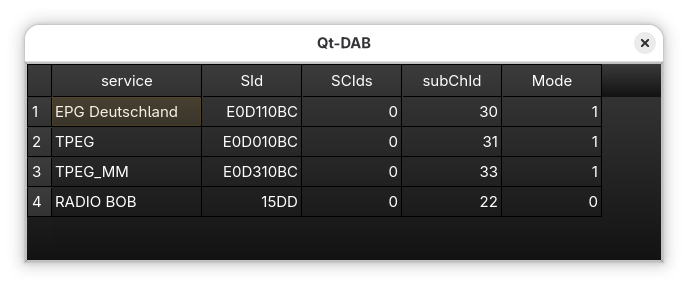
\includegraphics[width=110mm]{background-table.png}
\end{center}
In this example, the table shows that 4 services are running. The foreground service is marked with Mode 0, the background services with Mode 1.
\par
Clicking with the mouse on a background service, either automatically started or by the user, stops that service.
\section{The ensemble list}
As mentioned, ensemble lists are maintained between program invocations. The
default list is stored and an xml encoded file in the directory {\em serviceLists}, stored in the Qt-DAB-files-7 directory in the home directory.
\par
Setting the selector labeled {\em load selection} tells Qt-DAB that on the next (re)start you want to choose among a number of options for selecting a serviceList

\begin{center}
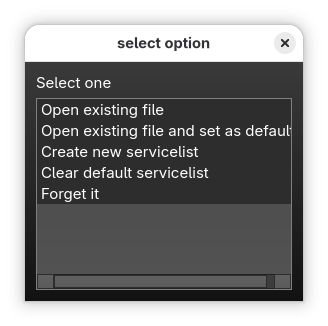
\includegraphics[width=80mm]{selectionload.png}
\end{center}
The options are 
\begin{enumerate}
\item {\em Open an existing file}. Apparently in a previous session a named servicelist was created and in the fortcoming session its data is used;
\item {\em Open an existing file and set as default}. Apparently in a previous session a servicelist was created and from now on it should be used as the default one (The original default one will just remain to exist);
\item {\em Create new servicelist}, i.e. an empty file will be created that is used during this program invocation as "the" servicelist.
\item {\em Clear the default servicelist}, with the obvious meaning;
\item {\em Forget it} just in case you have econd thoughts, in the coming session the default list is used.
\end{enumerate}
\end{document}
